\documentclass[11pt,a4paper,notitlepage]{article}

% Input encoding
\usepackage[utf8]{inputenc}
\usepackage[T1]{fontenc}  		% nur gemeinsam mit lmodern!
\usepackage{lmodern}
\usepackage{ngerman}

\usepackage{amsmath}
\usepackage{amsfonts}
\usepackage{amssymb}

\usepackage{booktabs}
\usepackage{supertabular}

\usepackage[pdftex]{graphicx}

\usepackage[pdfauthor={Wincent Balin},
            pdftitle={Befragung zur Bedienung von Pro Tools mit Mausgesten}]{hyperref}

\author{Wincent Balin}
\title{Befragung\\zur Bedienung von \emph{Pro Tools}\\mit Mausgesten}

\begin{document}
\maketitle

Die Befragung wird durchgeführt, um für die Möglichkeiten, ein DAW-Programm mit Gesten zu bedienen, Vorschläge zu sammeln.
Die zur Wahl stehende Gesten finden Sie in der nachfolgenden Tabelle.

\newcommand{\quarterpic}[1][]{\includegraphics[scale=0.25]{img/#1}}
\tablelasttail{\bottomrule}
\begin{center} \label{tab:Gestures}
\tablefirsthead
{
  \toprule
  Nummer & Darstellung & Erklärung \\ \cmidrule(r){1-1} \cmidrule(lr){2-2} \cmidrule(l){3-3}
}
\tablehead
{
  \toprule
  \multicolumn{3}{@{}l}{\small Fortsetzung} \\ \midrule
  Nummer & Darstellung & Erklärung \\ \cmidrule(r){1-1} \cmidrule(lr){2-2} \cmidrule(l){3-3}
}
\tabletail
{
  \midrule
  \multicolumn{3}{@{}r}{\small Fortsetzung folgt} \\ \bottomrule
}
\bottomcaption{Verfügbare Gesten}
\begin{supertabular}{rcl}
  1 & \quarterpic[right] & Bewegung nach rechts \\
  2 & \quarterpic[right-up] & Bewegung nach rechts, dann nach oben \\
  3 & \quarterpic[right-down] & Bewegung nach rechts, dann nach unten \\
  4 & \quarterpic[right-left] & Bewegung nach rechts, dann nach links \\
  5 & \quarterpic[right-left-right] & Bewegung nach rechts, dann nach links, rechts \\
  6 & \quarterpic[left] & Bewegung nach links \\
  7 & \quarterpic[left-right] & Bewegung nach links, dann nach rechts \\
  8 & \quarterpic[left-right-left] & Bewegung nach links, dann nach rechts, links \\
  9 & \quarterpic[up-down-up] & Bewegung nach oben, dann nach unten, oben \\
 10 & \quarterpic[down-left] & Bewegung nach unten, dann nach links \\
 11 & \quarterpic[down-right] & Bewegung nach unten, dann nach rechts \\
%  1 & 
\includegraphics[scale=0.25]{img/up} & Bewegung nach oben \\
%  2 & 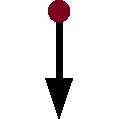
\includegraphics[scale=0.25]{img/down} & Bewegung nach unten \\
%  3 & 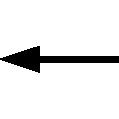
\includegraphics[scale=0.25]{img/left} & Bewegung nach links \\
%  4 & 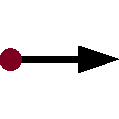
\includegraphics[scale=0.25]{img/right} & Bewegung nach rechts \\
%  5 & 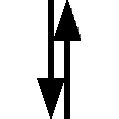
\includegraphics[scale=0.25]{img/up-down} & Bewegung nach oben, dann nach unten \\
%  6 & 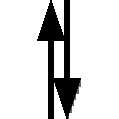
\includegraphics[scale=0.25]{img/down-up} & Bewegung nach unten, dann nach oben \\
%  7 & 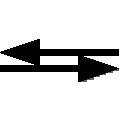
\includegraphics[scale=0.25]{img/left-right} & Bewegung nach links, dann nach rechts \\
%  8 & 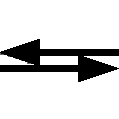
\includegraphics[scale=0.25]{img/right-left} & Bewegung nach rechts, dann nach links \\
%  9 & 
\includegraphics[scale=0.25]{img/up-down-up} & Bewegung nach oben, dann nach unten, oben \\
% 10 & 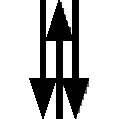
\includegraphics[scale=0.25]{img/down-up-down} & Bewegung nach unten, dann nach oben, unten \\
% 11 & 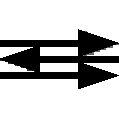
\includegraphics[scale=0.25]{img/left-right-left} & Bewegung nach links, dann nach rechts, links \\
% 12 & 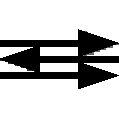
\includegraphics[scale=0.25]{img/right-left-right} & Bewegung nach rechts, dann nach links, rechts \\
\end{supertabular}
\end{center}

Tragen Sie bitte in die nachfolgende Tabelle die Nummern der Ihrer Ansicht nach geeignetsten Gesten
in die rechte Spalte ein. Einträge von mehreren Gestennummern sind erlaubt. Beim Eintragen von mehreren
Gestern gilt die zuerst eingetragene als die am meisten geeignete, die nachfolgende als die weniger geeignete
und so weiter.

Sie können in dem Fall, wenn Ihnen eine in der vorausgehenden Tabelle nicht aufgeführte Geste am geeignetsten
erscheint, zuerst diese Geste in eine der dafür frei gelassenen Zeilen mit Nummer eintragen und dann diese
Geste in der nachfolgenden Tabelle angeben.

\begin{center} \label{tab:Functions}
\tablefirsthead
{
  \toprule
  Deutsche     & Englische    & Tasten- & Gesten-        \\
  Bezeichnung  & Bezeichnung  & kombi-  & vorschlag      \\
  der Funktion & der Funktion & nation  & (ggf. mehrere) \\ \cmidrule(r){1-1} \cmidrule(lr){2-2} \cmidrule(lr){3-3} \cmidrule(l){4-4}
}
\tablehead
{
  \toprule
  \multicolumn{4}{@{}l}{\small Fortsetzung} \\ \midrule
  Deutsche     & Englische    & Tasten- & Gesten-        \\
  Bezeichnung  & Bezeichnung  & kombi-  & vorschlag      \\
  der Funktion & der Funktion & nation  & (ggf. mehrere) \\ \cmidrule(r){1-1} \cmidrule(lr){2-2} \cmidrule(lr){3-3} \cmidrule(l){4-4}
}
\tabletail
{
  \midrule
  \multicolumn{4}{@{}r}{\small Fortsetzung folgt} \\ \bottomrule
}
\bottomcaption{\emph{Pro Tools}-Funktionen}
\begin{supertabular}{llll}
 & & & \\
\end{supertabular}
\end{center}

\end{document}
